\chapter{Wyniki}
\label{cha:wyniki}

\section{Wydajność}
\label{sec:wydajnosc}
Poniżej zostaną zaprezentowane przykładowe wyniki czasu działania algorytmu dla odpowiednio wierszy od góry dwóch procesorów oraz dwóch kart graficznych. 
\begin{table}[h]
\resizebox{\textwidth}{!}{%
\begin{tabular}{|c|c|c|c|c|c|c|c|}
\hline
Unit \textbackslash data size ($n$)                                          & 10    & 50    & 100   & 150   & 250    & 400   & 1000 \\ \hline
\begin{tabular}[c]{@{}c@{}}i7 4710HQ\\ (4 cores)\end{tabular}           & 131ms & 2.6s  & 51s   & 4m7s  & -       & -      & -     \\ \hline
\begin{tabular}[c]{@{}c@{}}i7 7700HQ \\ (4 cores)\end{tabular}          & 112ms & 2.9s  & 40s   & 3m22s & 26m55s & -      & -     \\ \hline
\begin{tabular}[c]{@{}c@{}}GTX 850m \\ (640 cuda cores)\end{tabular}    & 121ms & 0.22s & 1.25s & 5.69s & 45s    & 5m30s & -     \\ \hline
\begin{tabular}[c]{@{}c@{}}GTX 1070m \\ (2048 cuda cores)\end{tabular} & 439ms & 0.19s & 0.41s & 4.86s & 57s    & 4m30s & 71m  \\ \hline
\end{tabular}%
}
\caption{Czas obliczeń dla poszczególnych układów dla 4 wymiarowego zbioru danych o n elementach.}
\end{table}
Czas działania programu powinien być porównywany w jednej kolumnie, ponieważ ilość kroków do osiągnięciu odległości międzyklastrowej będzie zależeć od danych.
Tabela została jedynie częściowo wypełniona ze względu na czas obliczeń wymagany do uzyskania rezultatów. Niepokojąco może wyglądać kolumna dla 10-cio elementowych danych, gdzie teoretycznie najbardziej wydajna jednostka uzyskuje najdłuższy czas działania. Mogłoby być to spowodowane chwilowym zajęciem układu przez inne zadanie. Najbardziej miarodajne rezultaty do porównania procesora z kartą graficzną dają większe zbiory danych. Szacunkowy czas działania CPU dla 1000 elementowych danych wynosiłby około 50 godzin.

\begin{figure}[H]
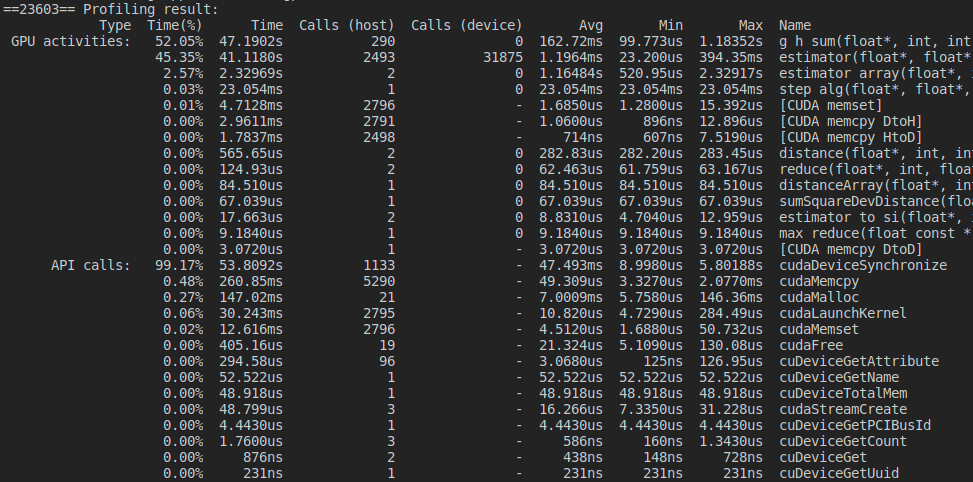
\includegraphics[width=\textwidth]{img/nvprof250}
\caption{Wyniki profilera cuda dla zbioru 250 el.}
\end{figure}
Jak wydać ze zrzutu powyżej czas obliczeń rozłożony jest głównie między funkcje liczące estymator oraz $g(h)$. O ile przy estymatorze nie ma dużych możliwości poprawy czasu działania, o tyle w przypadku metody doboru parametru wygładzania istnieją metody mniej złożone obliczeniowo. Metoda krzyżowanego uwierzytelniania (ang. cross-validation) może zostać zastąpiona metodą podstawień (ang. plug-in) bądź nawet metodą przybliżoną \cite{Kul05} co znacząco zmniejszy udział czasu wyliczania parametru $h$ w algorytmie.

\section{Jakość}
\label{sec:jakosc}
W niektórych przypadkach działanie algorytmów nie jest ze sobą tożsame. Jest to spowodowane niepoprawnym wyznaczeniem parametru h dla tablicy odległości. Skutkuje to różną odległością międzyklastrowa i w konsekwencji różną liczbą klastrów. Podczas liczenia minimum funkcji $g(h)$ różnice w wynikach na 4, 5, 6 miejscu po przecinku odgrywają kluczową rolę w części zbiorów danych. Błąd powstaje w wyniku asynchronicznego sumowania znaczącej liczby elementów, gdzie błąd numeryczny kumuluje się w czasie. Możliwym rozwiązaniem problemu jest zmiana precyzji obliczeń z pojedynczej na podwójną. Stworzy to kolejny problem wydajnościowy, gdyż stosunek jednostek podwójnej do pojedynczej precyzji w jednostkach konsumenckich wynosi 1:32. Co prawda istnieją układy jak GV100 posiadające bardziej korzystny stosunek 1:2, lecz są to jendostki spotykane głównie w klastrach obliczeniowych. Innym rozwiązaniem mogłoby być użycie innej metody wyznaczania parametru wygładzania, lecz będzie to tylko odkładaniem w czasie problemu, który i tak wyjdzie przy estymatorze dla większego zbioru danych.